\chapter{Projekt Smart Factory-Anlage}\label{ch:data}

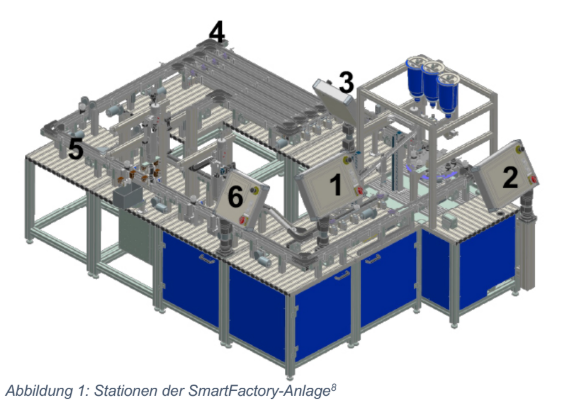
\includegraphics{figures/Screenshot 2025-01-03 124137.png}

\section{Projekt Smart Factory-Anlage: Aufgabenstellung (evtl noch umschreiben)}\label{sec:Projekt Smart Factory-Anlage: Aufgabenstellung (evtl noch umschreiben)}

Die SmartFactory-Anlage ist eine speziell für Schulungszwecke konzipierte
Automatisierungsanlage, die von der Abteilung Expert House entwickelt wurde. Sie beinhaltet verschiedene Produkte aus dem Siemens-Produktkatalog wie zum Beispiel speicherprogrammierbare Steuerungen, Lichtsensoren und Motoren.
Meine Aufgabe bestand darin, zusammen mit 18 weiteren Studierenden die
Weiterentwicklung für diese Anlage durchzuführen. Dies umfasste sowohl die
vollständige Ausbesserung von Bugs, als auch das Testen der Robustheit der Software. Die Software wurde nach dem ISA-88-Standard umgesetzt und alle Erweiterungen sollen auch nach diesem hinzugefügt werden. Zur Programmierung war die Siemens-Automatisierungssoftware „TIA-Portal“ zur Verwendung vorgegeben. Eine weitere Anforderung war es, die umfassenden Dokumentationsunterlagen in Form von Word-Dokumenten für nachfolgende Studierende auszubessern und gegebenenfalls mit den neuen Funktionen zu erweitern. Die Nutzung des ISA-88-Standard soll gewährleisten, das die Anlage ohne einen Ansprechpartner aus unserem Projektteam weiterentwickelbar ist. 
(evtl auf aufteilung unit,em,cm eingehen?)


\section{Projekt Smart Factory-Anlage: Zielsetzung}\label{sec:Projekt Smart Factory-Anlage: Zielsetzung}

Das Ziel am Ende des Praxissemesters war es, die funktionsfähige
SmartFactory-Anlage Weiterzuentwickeln, ihre Robustheit zu erhöhen und dies zu präsentieren. Dafür muss für jedes Anlagenmodul bekannte Fehler und offene Punkte aus der LOP abgearbeitet werden, sowie bei der erkennung neuer Fehler, diese zur LOP hinzugefügt werden. Desweiteren müssen die Bedingungen des Projektowners, eine einheitliche HMI-Schnittstelle und eine leichte Bedienung der Anlage umgesetzt werden.

(Maybe auf zyklische kommunikation und buggfixes eingehen? Teil der Zielsetzung?: Bei der SmartFactory-Anlage handelt es sich eine Übungs- und Testanlage zu Ausbildungszwecken und dem Testen von Prototypen. Sie simuliert eine Flaschenabfüllungsproduktion in einem kleinen Format und soll Auszubildenden mit vielen Produkten aus dem Siemens-Katalog vertraut machen.
Die Anlage ist daher in sechs Anlagenmodule unterteilt, von der Materialzuführung bis hin zum abschließenden Recycling, jedes mit verschiedenen Schwerpunkten aber ähnlicher Hardware. Hardwaretechnisch sind alle Anlagen mit einer Siemens-
Simatic S7-1500 Speicherprogrammierbaren Steuerung, sowie einem Siemens-
HMI, einem Touchscreen für Statusmeldungen und Benutzereingaben und Transportbändern ausgestattet. Desweiteren sind an einigen Stationen pneumatisch betreibende Greifern und RFID-Schreib-Lesegeräte verbaut. Die Anlage läuft iterativ. Im Falle der Anlage bedeutet dies, dass am Ende des Kreislaufes, nach dem Recycling, die Flaschen, Deckel und Kugeln wieder für die erneute Verarbeitung bereitgestellt werden, damit sie erneut abgefüllt werden können. Die Anlage kann über drei Betriebsmodi, Einrichtungs-, Hand- und Automatikbetrieb und zwei Betriebsarten, Modular- und Inselbetrieb über das stationszugehörigen HMI gesteuert werden. Im Einrichtungsbetrieb kann der Bediener uneingeschränkt alle Anlagenteile bewegen, auch wenn dies zu mechanischen Fehlern führen könnte. Der Handbetrieb ermöglicht es, einzelne Funktionen, die sich aus der Ansteuerung mehrerer Aktoren zusammensetzen auszuführen, beispielsweise das Befüllen einer Flasche oder das Entleeren eines Bandes. Im Automatikbetrieb soll die Anlage vollständig automatisiert laufen und nur im Fehlerfall oder zum Anlegen eines Auftrags einen Bediener erfordern. Im Folgenden wird der Ablauf der verschiedenen Stationen der Anlage im Automatikbetrieb erläutert.)

noch teil der Zielsetzung?

Maybe als kurzbeschreibung der Anlage?

\subsection{Station 1: Modulares Produktionssystem (umschreiben)}\label{sec:Station 1: Modulares Produktionssystem (noch umschreiben)}

Das Modulare Produktionssystem nimmt Flaschen und Deckel von der Recycling-Anlage entgegen und stellt diese auf Anforderung 
der Abfüllstation zur Verfügung. Sie leitet nur weiße Deckel weiter, während deckel mit einer anderen farbe aussortiert 
werden. Deckel mit unlesbaren RFID-Tag sollen grundsätzlich aussortiert werden. Sollte eine Anforderung der Abfüllstation 
erfolgen, wird die angegebene Anzahl der Flaschen gesendet und bei Anforderung ein Deckel auf die befüllte Flasche gesetzt.

\subsection{Station 2: Abfüllung (geschrieben)}\label{sec:Station 2: Abfüllung (selber geschrieben)}

Die Abfüllstation hat die Aufgabe, Flaschen mit einer vorgegebenen Anzahl von Kugeln zu befüllen. Diese Anzahl wird durch 
die Erstellung von Aufträgen am HMI festgelegt. Hier kann zum Beispiel der Prozentsatz der Kugelfarbe (bei einem Maximum 
von 250 Kugeln) oder ein Absolutwert für die Anzahl der Kugeln festgelegt werden. Für das abfüllen, hat die Abfüllung drei 
Container mit jeweils, roten, blauen und gelben Kugeln. Außerdem kann die Anzahl der abzufüllenden Flaschen angegeben 
werden. Diese Anzahl wird per "On-Demand"-TCP-Verbindung an das modulare Produktionssystem gesendet. Die danach von dem 
modulare Produktionssystem gesendeten Flaschen werden durch einen Drehteller an verschiedenen Verarbeitungsstationen bewegt. 
Als erstes wird die Flasche mit des Auftrages angegebenen Anzahl an Kugeln befüllt. Dann wird ein Deckel von dem modulare 
Produktionssystem angefordert. Der Deckel wird danach mit einen drehbaren Greifer verschraubt und an der nächsten Station 
wird der Deckel mit einem RFID-Tag beschrieben. Der RFID-Tag enthält Datum und Uhrzeit der Abfüllung, sowie welcher Auftrag 
abgefüllt wurde.

\subsection{Station 3: Quality Gate (geschrieben)}\label{sec:Station 3: Quality Gate (selbst geschrieben)}

Das Quality Gate soll wie der Name sagt, die Auftragsdaten auf dem RFID-Tag mit dem Inhalt der Flasche abgleichen. Hierzu 
soll ein Farbsensor dienen, der die farbliche Zusammensetzung prüft. Sollte die farbliche Zusammensetzung übereinstimmen, 
wird der RFID-Tag der Flasche mit “Gut” beschrieben, sollte sie aber nicht übereinstimmen wird der RFID-Tag mit “„Ausschuss” 
beschrieben.

\subsection{Station 4: Kommissionierbahnen (geschrieben)}\label{sec:Station 4: Kommissionierbahnen (selbst geschrieben)}

Die Kommissionierbahnen sollen die vom Quality-Gate ankommenden Flaschen nach Auftragsnummer sortieren, hierzu wird zu 
beginn der RFID-Tag gelesen und die Flasche auf eine von vier Bahnen sortiert. Fehlerhafte Flaschen werden direkt über ein 
Ausschussband an die nächste Station weitergegeben. Sollte die Flasche “In Ordnung” sein, wird sie auf eine von vier Bändern 
sortiert. (ein auftrag pro band). Die sortierten Flaschen sollen so lange in der Station gehalten werden,
bis der entsprechende Auftrag abgeschlossen wurde oder der Bediener ein
manuelles Entleeren der Bänder anfordert.

\subsection{Station 5: Eckstation (geschrieben)}\label{sec:Station 5: Eckstation (selbst geschrieben)}

Das Feature der Eckstation ist, zwei Laufbänder, die wie hochklappbare Brücken fungieren. Das Hochklappen ermöglicht es, 
einen Schaltschrank in der Mitte der Anlage zu erreichen. Das Hochklappen der Laufbänder soll unterbunden werden, wenn 
noch Flaschen auf dem Laufband sind. Dies erfordert das Tracken der Flaschenanzahl und einen Stopper, um den Zulauf der 
Flaschen bei hochgeklappten Laufbändern zu verhindern und das Hochklappen bei vollem Laufband zu verhindern. Ist das 
Laufband voll, wird der Zulauf durch den Stopper verhindert.

\subsection{Station 6: Recycling (geschrieben)}\label{sec:Station 6: Recycling (selbst geschrieben)}

Die Recyclingstation recycelt alle ankommenden Flaschen, also alle aus erfolgreich erfüllten Aufträgen und alle aussortierten
Flaschen. Der Flaschendeckel wird mit einem Greifer entfernt und auf ein anderes Laufband gesetzt. Danach wird die Flasche 
angehoben und die Kugeln über einem Trichter entfernt. Die Kugeln werden daraufhin mit einem Farbsortierer und Luftdruck in 
die farblich übereinstimmenden Container an der Abfüllung geschossen, und die Flasche wird auf das Laufband zum modularen 
Produktionssystem gesetzt.

\subsection{Netzwerkverbund (geschrieben)}\label{sec:Netzwerkverbund: (selbst geschrieben)}

Alle Anlagenteile sind mit Ethernet mit dem Einschaltschrank verbunden und bilden damit ein Subnetz. Dies ermöglicht eine 
effiziente und stabile Kommunikation zwischen den verschiedenen Stationen der Anlage und ermöglicht das senden und empfangen 
von Daten.
Die gesamte Kommunikation der Anlage erfolgt “On-Demand” und passiert dadurch nur wenn sie von einer anderen Station 
angefordert wird. Dies minimiert unnötigen datenverkehr und trägt dadurch zur Reduzierung der verbrauchten Ressourcen bei.

\section{Projekt SmartFactory-Anlage: Projektorganisation (geschrieben)}\label{sec:Projekt SmartFactory-Anlage: Projektorganisation (am ändern)}

Das Projektteam besteht aus ... Informatikstudenten und ... Elektro- und Informationstechnikstudenten sowie drei 
Fachbetreuern. Diese haben uns als "Product Owner" im Projekt unterstützt und geleitet.  

Das gesamte Projekt wurde auf Scrum basierend durchgeführt. Allerdings wurde, wie in Abschnitt 1, "Einleitung", erläutert, 
sowohl bei uns, den Informatikern, als auch bei den Elektro- und Informationstechnikern, die Phase im Expert House durch die 
SPE-Phase unterbrochen, dies allerdings zu unterschiedlichen Zeitpunkten. Dadurch wurde in den ersten acht Wochen von allen 
gemeinsam am Projekt gearbeitet, in den folgenden acht Wochen nur von den Elektro- und Informationstechnikern, und in den 
letzten acht Wochen ausschließlich von uns Informatikern.  

Dies führte dazu, dass an den Übergabepunkten große und kleine Änderungen klar an die "Nachfolger" übergeben werden mussten.
Gleichzeitig war es essenziell, die Dokumentation stets auf dem aktuellen Stand zu halten, um eine reibungslose Weiterarbeit 
zu ermöglichen.  

Dies passte gut, da wir unser Team mit Scrum organisiert haben. Dadurch stimmten wir uns gemeinsam, Betreuer und 
Auszubildende, in Daily-Meetings ab. Wir arbeiteten in Zwei-Wochen-Sprints, die jeweils mit einer Vorstellung der 
Ergebnisse an die Stakeholder endeten. Eine zentrale Rolle spielte die "List of Open Points" (LOP), die zur Dokumentation 
von bestehenden Fehlern und Mängeln genutzt wurde.  

Die LOP war in Dringlichkeitsstufen unterteilt:
\begin{itemize}
    \item \textbf{Sehr wichtig:} Prozessbeendende Fehler oder solche, die mechanische Schäden verursachen könnten.
    \item \textbf{Mittel:} Fehler, die den Prozess nicht vollständig stoppen, aber zu Fehlern in der Verarbeitung von Flaschen führen.
    \item \textbf{Niedrig:} Fehler mit geringeren Auswirkungen, z. B. das Herausfallen einer Kugel bei der Initialisierung der Abfüllstation.
\end{itemize}


Die Stakeholder legten diese Prioritäten fest. Für jeden Sprint suchten sich die Verantwortlichen der jeweiligen Station 
die wichtigsten Aufgaben mit der höchsten Priorität heraus und arbeiteten diese ab.  

Gerade zu bearbeitende Aufgaben und bereits abgeschlossene wurden in ein Kanban-Board eingetragen. Dies half, den Fortschritt 
zu visualisieren und machte in den Daily-Meetings deutlich, welche Aufgaben eventuell vom Plan abwichen. Dadurch konnten 
notwendige Anpassungen schnell besprochen und vorgenommen werden, um weiterhin das Projektziel in der gegebenen Zeit zu 
erreichen.  

Obwohl wir uns nicht strikt an Scrum hielten, ergab dieser Ansatz aus unserer Sicht Sinn. Der Überblick über die aktuellen 
Aufgaben war so deutlich besser, und die Verständlichkeit in den Meetings wurde durch die Visualisierung wesentlich 
erleichtert.

Das Kanban-Board wurde in folgende Bereiche unterteilt:
\begin{itemize}
    \item \textbf{Aufgaben:} Hier befinden sich alle Aufgaben, die im aktuellen Sprint erledigt werden müssten, mit denen sich aber noch niemand befasst hat.
    \item \textbf{In Bearbeitung:} Hier wurden die aktuell bearbeiteten Aufgaben gesammelt.
    \item \textbf{Internes Review:} Wurde eine Aufgabe abgeschlossen, wurde das Ergebnis zunächst durch einen weiteren Studierenden überprüft.
    \item \textbf{Ready for Review:} Eine von einem Studierenden als in Ordnung befundene Aufgabe wird noch ein weiteres Mal durch einen Betreuer geprüft.
    \item \textbf{Nacharbeiten:} Wurde eine durchgeführte Aufgabe entweder von einem Betreuer oder einem Studierenden als nicht in Ordnung befunden, oder es traten im Projektverlauf Probleme damit auf, ist sie in diesem Bereich zu finden.
    \item \textbf{Erledigt:} In diesem Bereich befinden sich schließlich komplett abgeschlossene Aufgaben.
\end{itemize}

\section{Projekt SmartFactory-Anlage: Projektverlauf (umschreiben)}

\textbf{"Begriffsklärung „TIA Portal“:"}

Im nachfolgenden Abschnitt wird das TIA-Portal mehrfach thematisiert. Dabei handelt es sich um die 
Entwicklungsumgebung für alle Automatisierungsprodukte von Siemens \cite{bee2022}.



Die Prozesslogik für SPS (Speicherprogrammierbare Steuerungen) kann in unterschiedlichen Programmiersprachen, unter 
anderem FUP, AWL und SCL, programmiert werden. Die SmartFactory-Anlage sollte bedarfsgerecht in FUP (Funktionsplan) und SCL 
(Structured Control Language) programmiert werden. Da es sich bei einer PLC um ein Echtzeitsystem handelt, welches zyklisch 
arbeitet, müssen bei der Programmierung einige Aspekte berücksichtigt werden. Hierzu stehen folgende Konzepte zur Verfügung:

\begin{itemize}
    \item \textbf{Funktion:} Vergleichbar mit einer Methode, beispielsweise in C\#. Eine Funktion kann Übergabeparameter verarbeiten und darauf basierende Ausgabewerte berechnen. Allerdings werden die Ausgabewerte in jedem Programmzyklus neu berechnet und sind somit nicht persistent.
    \item \textbf{Funktionsbaustein:} Bietet die gleiche Funktionalität wie eine Funktion, mit dem Unterschied, dass Daten über einen Zyklus hinaus gespeichert werden.
    \item \textbf{Datenbaustein:} In einem Datenbaustein werden für das Programm notwendige Daten persistent gespeichert. Bei der Erstellung eines Funktionsbausteins wird ebenfalls ein Datenbaustein für dessen Daten angelegt.
    \item \textbf{User Defined Datatype (UDT):} Ein vom Programmierer festlegbarer Datentyp.
\end{itemize}

